%!TEX program = xelatex
\documentclass[border=10pt]{standalone}
% \usepackage{xeCJK}
% \usepackage{fontspec}
\usepackage{inputenc}
\usepackage{tikz}
\usetikzlibrary{shapes.geometric, arrows, shapes.symbols}

\tikzstyle{arrow} = [thick,->,>=stealth]
\tikzstyle{block} = [rectangle, draw, text centered, rounded corners, minimum height=2em]
\tikzstyle{pipe} = [cylinder, draw, shape border rotate=0, aspect=0.3, 
minimum height=8em, minimum width=2em, fill=blue!50]

\begin{document}

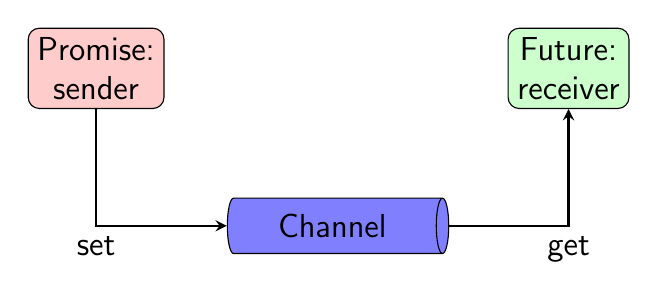
\begin{tikzpicture}[node distance=2.5cm, font=\sffamily\large]
    % Nodes
    \node[block, align=center, fill=red!20] (promise) at (0,  0) {Promise:\\ sender};
    \node[pipe,  align=center] (channel) at (3, -2) {Channel};
    \node[block, align=center, fill=green!20] (future)  at (6,  0) {Future:\\ receiver};

    % Arrows
    \draw[arrow] (promise.south) |- (channel.west) node[midway, below] {set};
    \draw[arrow] (channel.east) -| (future.south) node[midway, below] {get};

\end{tikzpicture}

\end{document}